\graphicspath{{figures/appendix-SDSup/}}

\chapter{SUNIST 数据采集与处理服务系统(SDSup)}

\section{SUNIST 数据采集系统升级的目的与意义}

SUNIST 装置建成时,采用的数据采集系统(WLYXZ)\cite{}由两台 16 通道数据采集机箱组成。最高采样速率可达 $5\,{\rm MSPS}$,每通道最高 $32\,{\rm kB}$ 存储空间。每次采集时,当各通道存储空间已满时停止采集,其工作框图在图 \ref{fig:chap04:wlyxz} 中画出。在 WLYXZ 系统中,采集数据被存储在二进制文件中,并基于文件系统进行管理与存储,不利于对历史实验数据的获取\pozhehao 必须先使用专用的只能运行在纯 DOS 系统的数据转换程序转换为文本文件。而且数据文件容易损坏,并且在 WLYXZ 系统中没有备份机制。

\begin{figure}%[H]
  \centering
  \fbox{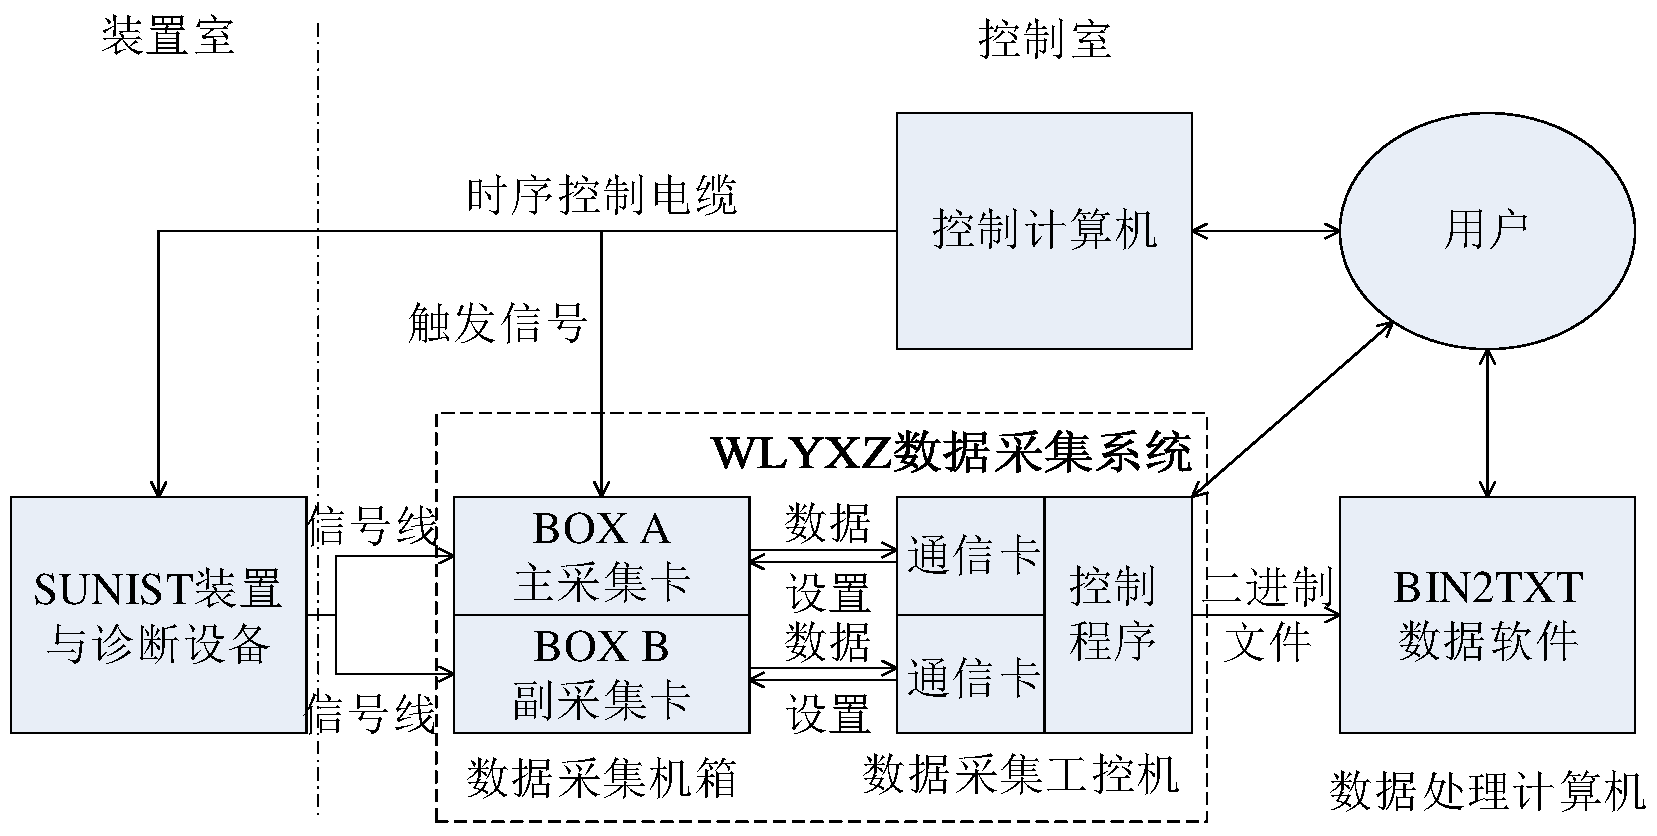
\includegraphics[width=\textwidth]{wlyxz.pdf}}
  \caption{SUNIST 旧数据采集系统 WLYXZ 框图}
  \label{fig:chap04:wlyxz}
\end{figure}

自 2008 年春季开始,SUNIST 装置开始进行升级改造,安装了多种诊断设备与系统。WLYXZ 系统不再满足 SUNIST 的数据采集需求,对数据采集系统的升级改造提上日程。升级后,SUNIST 数据采集与处理服务系统(SUNIST Data acquisition and processing Serving system Upgrade, SDSup)要求要具有:1)升级的信号采集能力,并提供可以随时连接 SUNIST 后续安装的诊断设备的能力;2)基于炮号进行数据管理、存储与备份,拥有可以长时间运行的系统软件环境;3)数据可以分布式访问,提供多种编程接口,为多人协作参与实验研究提供基础。

基于以上要求,SDSup 系统拟采用 MDSplus\cite{MDSplus:url,MDSplus:paper:1,MDSplus:paper:2} 数据库为核心建立。MDSplus 是专门为托卡马克实验研究开发的一套程序与工具的合集。具有数据存储、管理和访问以及实验控制功能,在国际聚变等离子体研究装置上使用非常广泛\cite{MDSplus:use:NSTX,MDSplus:use:EAST,MDSplus:use:TCABR}。MDSplus 的优势还在于其提供了非常丰富的编程语言接口(JAVA, Fortran, C/C++, Matlab/Octave, VB.NET, IDL 等),后期实验数据处理时,并且可以随时将添加处理结果和研究笔记。在 SUNIST 上只采用其数据库功能。

\section{SDSup 系统组成与工作流程介绍}

Fig 1 shows the whole structural design of the SUNIST data acquisition and data service system. The system has three main parts, data acquisition devices, data managing and service system and user clients. The experiment control and monitor computer controls SUNIST discharge sequence and triggers data acquisition devices by communication with the relay timers using the ZigBee/IEEE 802.15.4 protocol. The control and monitor computer gets and displays the acquired data on the screens one shot cycle.

\begin{figure}%[H]
  \centering
  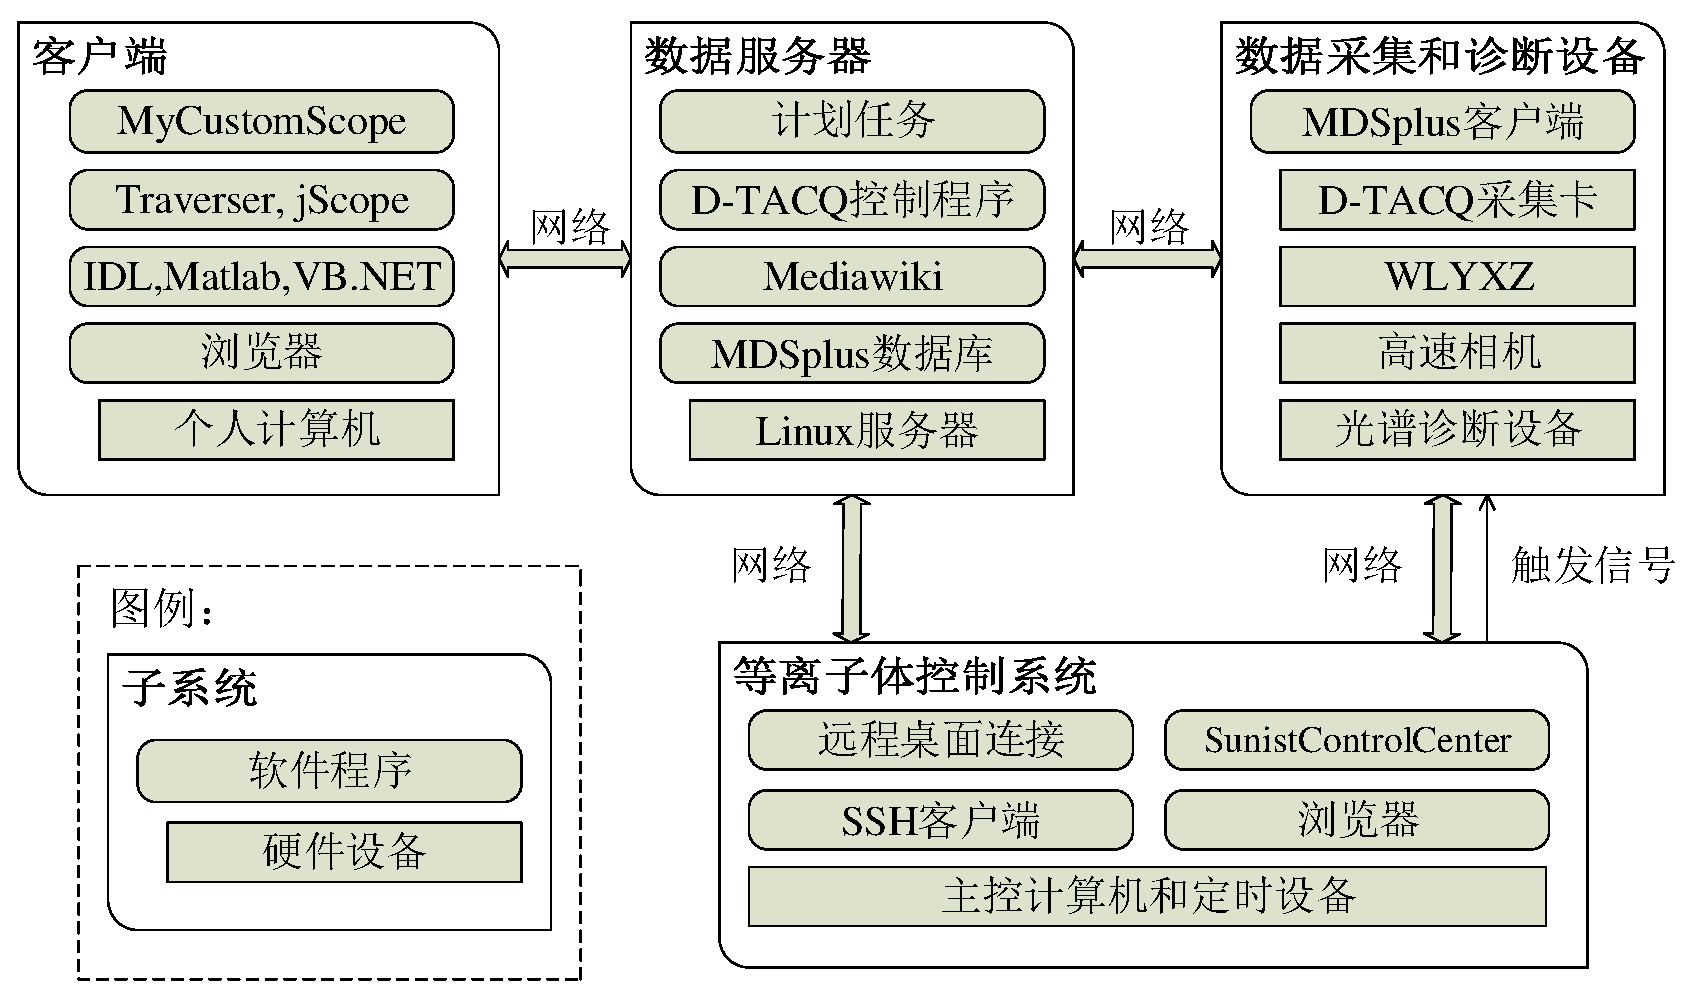
\includegraphics[width=\textwidth]{data-system-chs_cropped.pdf}
  \caption{升级后的 SUNIST 数据采集系统 SDSup 框图}
  \label{fig:chap04:SDSup-system}
\end{figure}

The data acquisition devices and data server form a separated network. And all the digitizers including WLYXZ, ACQ196 acquisition boards and other MDSplus client applications are all connected to the data server by a router. The SUNIST main server, which provides WWW, VPN and DNS services, tunnels the data server to internet then the laboratory users and operation monitor computer can retrieve the stored data on the data server and store analyzed data back to the server. It is a security improvement that the tunneling network framework shields the data server from the internet. The data server has four Inter Xeon X3220 CPU processer cores and 4GBytes memory and runs Ubuntu/Linux operation system. We develop a RAID1 hard disk array as the main storage for the data server to backup all the data into a mirror disk.

The WLYXZ digitizers have a 16-channel main box and a 16-channel slave box with 12-bit ADCs. The maximum sample rate is 5M samples per second (SPS). There are seven sample intervals: 0.2μS, 0.5μS, 1μS, 2μS, 4μS, 8μS and 16μS. The sampling rate is set by the data acquisition software. The ACQ196CPCI 96 channel digitizer board has true differential simultaneous analog input with 16-bit ADC for each channel. The two available sampling speeds are 250kSPS and 500kSPS. The ACQ196 slot has a 400MHz RSIC processor, runs embedded Linux and provides a MDSplus client application. The ACQ196 slot has several command and monitoring interfaces. We use the web interface for general status diagnostics and ssh interface for developing slot initiate and close control shell scripts on the data server.

During the first phase of discharge, the control and monitor computer ‘tells’ the MDSplus data server to create a new shot tree for the current shot data storage and charges the magnets field coils’ capacitors. When the shot begins, the data acquisition digitizers will be triggered first, and then the capacitors are discharged, at the same time all the inputs to digitizers will be recorded. All the raw data will be uploaded to MDSplus data server. The post shot process for raw data begins after uploading completed and the monitor computer will display the important parameters during the shot.




\begin{figure}%[H]
  \centering
  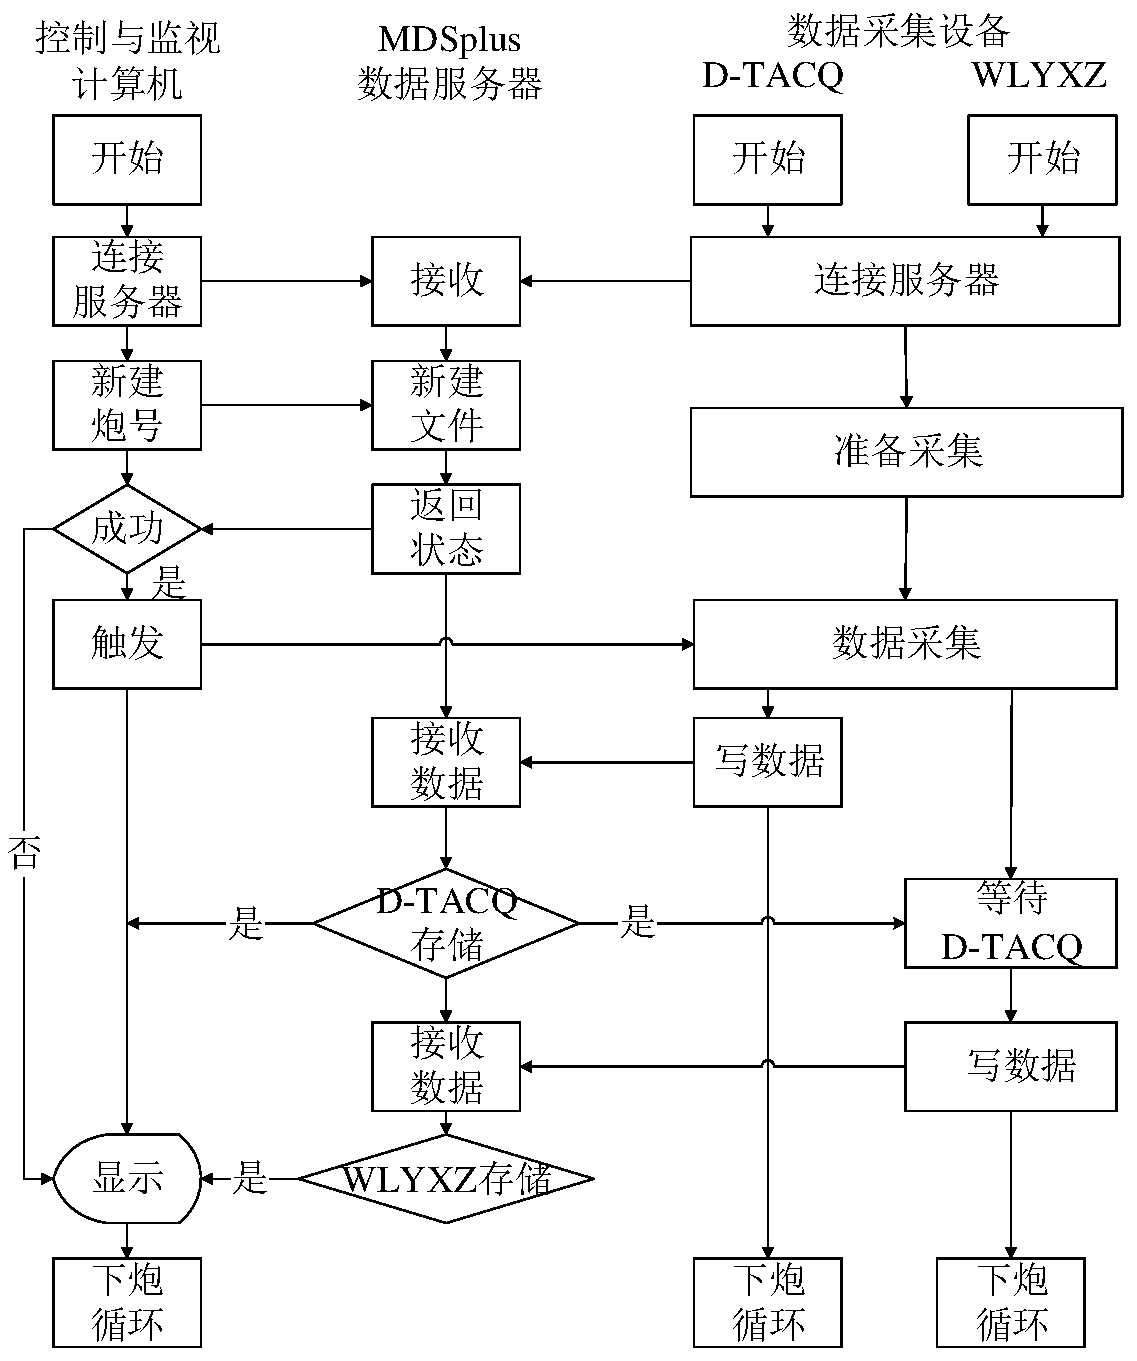
\includegraphics[width=0.7\textwidth]{SDSup-work-flow_cropped.pdf}
  \caption{SUNIST 数据采集与处理服务系统 SDSup 工作流程图}
  \label{fig:chap04:SDSup-work-flow}
\end{figure}

%\section{D-Tacq 数据采集板介绍}
%\section{SUNIST 新数据采集与处理服务系统}
\section{总结}
